\chapter{Methods}
\label{chapter:method}

%\section{Disambiguating Trees}
A shortcoming in the current probabilistic model used by the GF parser is that it is context free. As can be seen in figure \ref{fig:context_probs} the current model cannot use information such as the fact that in the phrase "eat bass", the word "bass" is much more likely to refer to the fish bass than the instrument bass, as each part of the tree is scored separately and independently of all other parts. The probabilistic model proposed is a way to use the ability to convert GF abstract syntax trees into abstract dependency trees in order to take context based information into account. Abstract dependency trees as introduced in \citep{kolachina2017ud2gf} are basically sense tagged dependency trees using feature, part of speech and dependency labels according to the Universal Dependencies scheme. 

The approach taken to disambiguation in this thesis is not a constructive approach in the sense that no focus is put on the parsing process and trying to \emph{find} the the correct abstract representation. Rather the approach taken is to develop a probabilistic model over \textbf{abstract dependency trees} able to score any abstract dependency tree according to the likelihood of that particular abstract dependency tree ocurring in natural text. This can then be used to evaluate parses done by the existing GF parser through conversion from abstract syntax to abstract dependencies and re-rank the k-best parses from the GF parser similar to what was done by \citet{kolachina2015GF} to improve disambiguation in the GF parser. A secondary application used as an evaluation task is general purpose word sense disambiguation on dependency parsed sentences.

The probabilistic model over abstract syntax tree is a syntactic n-gram model over the abstract functions (the word senses) in the ADT, where the probabilities of a tree only depends on its subtrees of the form of one node and its (n-1) immediate ancestors. Parameters for the statistical model is estimated from a large amount of text in several different languages parsed with UD-pipe. There is no need for sense tagged training data or parallel corpora. To circumvent the need for sense tagged data, the sense tags are treated as latent information in the text and Expectation Maximization is used together with a knowledge source of the possible senses for each word in every language for parameter estimation. The knowlege sources used are the current GF dictionary, and synset information from the Open Multilingual Wordnet.

\section{Tree Probabilities}
%\begin{itemize}
%    \item In order to compare sentences we need to define the probability of a whole tree. 
%    \item Sentences that is nonsense should be given a very low probability 
%    \item Connect back to the description of different ambiguities in the theory chapter, how do we approach solving the problem of syntactical and lexical ambiguities.
%    \item Conditioning on head gives information about this
%    \item Connection to syntactic ngrams
%\end{itemize}


In implementation and experiments focus have been limited to exploration of syntactic bigrams only, mainly because of computational and memory complexity of the algorithm used for parameter estimation. In the bigram model used the probability for a tree $T$ is calculated by the following product:
\begin{equation}
    P(T)=P(N_0)\prod_{i=1}^{n} P(N_i|H(N_i))=P(R_T)\frac{\prod_{i=1}^{n} P(N_i,H(N_i))}{\prod_{i=1}^{n} P(H(N_i))},
\end{equation}
where $N_0$ is the root node of the tree and $H(N_i)$ is the head node of $N_i$. Information contained in each node could in addition to the abstract function in the node include the dependency relation of the node and in the work both probabilities taking into account the dependency label and probabilities not taking this into account have been considered.

As a baseline to make comparisons to the current probabilistic model used in the GF parser possible a unigram model have also been used in which the probability for a tree $T$ is calculated by the following product:
\begin{equation}
    P(T)=\prod_{i=0}^{n} P(N_i),
\end{equation}
that is a completely context free model where each node is assumed independent.






%\todo{We must describe the probability model in the following aspects:}
%We have a correspondence GF2UD, how does probabilities of UD trees generalize to GF trees.\\
%How do we define probabilities on UD trees by only looking at probabilities of sub trees.\\
%We can decide to only look at some information such as only lemma and part of speech.\\
%How do we combine our probabilities with current parser probabilities
\section{Parameter Estimation}
In order for the probabilistic model to be useful one needs accurate estimations of the probabilities $P(N_i,H(N_i)), P(N_i),P(H(N_i))$. Since there is very little data labeled with abstract functions available to do such estimations directly through a method like maximum likelihood, the estimation is done through the use of a knowledge source of possible linearizations of every abstract function and corpora of untagged but dependency parsed text in several different languages. The method used is based on Expectation Maximization and is described in terms of estimating probabilities for subtrees of arbitrary size. It shall later be seen that the method does not scale very well computationally or memory wise to larger sub trees, which is why experiments have been limited to subtrees of size two. % The core of the developed method is the parameter estimation. The estimation is done from large amount of textual data deemed to be representative for the type of texts the model is supposed to describe. The main problem in estimating the parameters is that while the model describes properties of the unambiguous abstract dependency trees we do not have a large amount of data of abstract trees that could be used for estimation, we only have ambiguous text or normal dependency trees in different languages where the complete abstract functions are unknown. However with the use of knowledge based resources such as dictionaries and wordnets we can identify what ambiguities there are and use unsupervised methods like the Expectation Maximization method to overcome this problem.
%The probability model used need to estimate the frequency of certain sub-trees occurring in the abstract dependency trees of the type of text modelled. The abstract dependency trees of a sentence is unknown, but if we have the dependency trees of each sentence and a list of possible function tags for each node in a dependency tree we can treat the function tagged sub-trees as latent information that can be marginalized in a maximum likelihood estimation using for example expectation maximization.

We assume that the set of all possible function tagged sub trees is known and finite and we denote it
\begin{equation*}
    F=\{y_i\}_{i=1}^N.
\end{equation*}
The set of possible untagged subtrees will depend on the language the subtrees are defined over and in this work which language a subtree is defined over is always assumed to be known. The set of possible untagged subtrees for each language $s$ is also assumed to be known and finite and is denoted
\begin{equation*}
    W_s=\{x_{si}\}_{i=1}^M.
\end{equation*}
Lastly we also assume that we for each language have knowledge of a \emph{possibility set}
\begin{equation*}
D_s\subseteq W_s \times F,
\end{equation*}
where $(x_{si},y_j)\in D_s$ if and only if $y_j$ is a possible function tagged subtree given the untagged subtree $x_{si}$. The possibility sets used in this work are mostly derived using Wordnets and are discussed further in section \ref{section:building_subtrees}. %As a simple example of such a possibility set, consider such a set defined over all subtrees of size one, e.g. over all words in the language, and all abstract lexical representations of size one, e.g. all synsets in the wordnet. Then $D_s$ would consist of all pairs This could be ta is the set of all tagged subtrees of size one, that is simply all possible functions which for example could be defined to be all GF-functions in a certain dictionary file, or all wordnet synsets, section \ref{section:building_subtrees} further describes how these sets are constructed in the experimental setup. 

In the estimation of parameters using data from one or several corpora or treebanks we consider a sequence of observations \begin{equation*}
    O=(X_i, s_i)_{i=1}^K, X_i\in W_{s_i},
\end{equation*}
and assume that to every subtree $X_i$ in the set, there is a fixed and pre-determined $Y_i\in F$ such that $(X_i,Y_i)\in D_{s_i}$. That is, we assume that there is one correct abstract representation for each observed subtree. However, these $Y_i$ are unobservable and thus unknown. $O$ is also called the observable information while the observable information together with the correct abstract representation are called the \emph{complete information}.

The goal is to calculate the probability of seeing a certain abstract representation and we denote the probability of seeing the subtree $y_i\in F$ as
\begin{equation*}
    P(Y=y_i)=\pi_i.
\end{equation*}
Our goal will be to estimate the parameters $\pi=(\pi_1, \pi_2,...)$. In order to facilitate the use of the Expectation Maximization algorithm we will also as a byproduct calculate the probability of a (untagged) subtree given that it has a certain abstract representation and we denote these probabilities 
\begin{equation*}
    P(X=x_{sj} | Y=y_i, s) = \phi_{sij}
\end{equation*}. 

\subsection{Using a Maximum Likelihood approach}
Using a Maximum-likelihood approach to estimate the parameters $(\pi, \phi)$ means that we need to find the maximum of

\begin{equation*}
P(\pi, \phi | O)=\frac{P(O | \pi, \phi)P(\pi, \phi)}{P(O)},
\end{equation*}
where $P((\pi, \phi))$ is our prior belief of $(\pi, \phi)$ and $P(O | (\pi, \phi)) = l(O,(\pi, \phi))$ is the likelihood function for the used data set. The problem at hand is to maximize this likelihood function with respect to the parameters .

Since we assume observations are independent the likelihood function for all observations will just be the product of the likelihood functions of each individual observation and we thus look at the likelihood function for each observation, that is $P(X | \pi, \phi)$, separately. Now by the law of total probability we have 

\begin{equation*}
\begin{split}
P(X=x_j | \pi, \phi) = &\sum_{i:(x_j,y_i)\in D_s}P(X=x_j,y_i | \pi, \phi) = \\
&\sum_{i:(x_j,y_i)\in D_s} P(X=x_j|y_i , \pi, \phi)P(y_i | \pi, \phi) = \\
&\sum_{i:(x_j,y_i)\in D_s}\pi_i\phi_{ij},
\end{split}
\end{equation*}
which can be calculated without knowledge of the value of $Y$, since that variable was mariginalized out. However, as we want to calculate the total likelihood of all the observations 
\begin{equation*}
P(O | \pi, \phi) = \prod_{n=1}^K P(X=x_{j(n)} |\pi, \phi) = \prod_{n=1}^K \sum_{i:(X_n,y_i)\in D_s(n)} \pi_i\phi_{ij(n)},
\end{equation*}
which unless the sets $D_s$ are shaped very nicely will quickly become computationally intractable to maximize as the number of observations get large. However, this is almost the problem formulation that the Expectation Maximization algorithm is designed to find approximate solutions to.

\subsection{Using Expectation Maximization}
Using the expectation maximization method we look at maximizing the log-likelihood for the observations $L(O,\pi,\phi)$, which becomes $L(O,\pi,\phi)=\sum \log (\sum \phi_{ji}^{s_i}\pi_i)$. Calling the complete parameter set $\theta = (\pi, \phi)$ in the expectation step we get the expression 
\begin{equation*}
\begin{split}
Q(\theta,\theta_{t-1})%&=\sum_{X\in O} E_{\theta_{t-1}}\left ( L(Y,\theta) | X \right )\\
&=E_{\theta_{t-1}}\left ( L(C,\theta) | O \right )\\
&= \sum_{n=1}^K \sum_{j=1}^N
L(X_n, y_j,\theta)
P(y_j|X,\theta_{t-1})\\
&= \sum_{s \in S} \sum_{i=1}^{N_s} \sum_{j=1}^M 
L(x_i,y_j,\pi,\phi)
c_{si}P(y_j|x_i,\theta_{t-1})\\
&= \sum_{s \in S} \sum_{i=1}^{N_s} \sum_{j=1}^M 
(\log(\phi_{sij}) + \log(\pi_j))
c_{si}P(y_j|x_i,\theta_{t-1}),
\end{split}
\end{equation*}
where $c_{si}$ denotes the count of the observations of the form $(x_i,s)$. By rewriting the conditional probability of $y_i$ given $x_i$ in terms of the parameters in our model
\begin{equation*}
\begin{split}
P(y_j|x_i,\theta_{t-1})
%&=\frac{P(x_i|y_j,\theta_{t-1})P(y_j,\theta_{t-1})}{P(x_i|\theta_{t-1})}\\
&=\frac{P(x_i|y_j,\theta_{t-1})P(y_j,\theta_{t-1})}
{\sum_{k:(x_i,y_k)\in D_s}P(x_i|y_k,\theta_{t-1})P(y_k,\theta_{t-1})}\\
&=\frac{c_{si}\phi^{t-1}_{sij}\pi^{t-1}_{j}}
{\sum_{k:(X_n,y_k)\in D_{s}}\phi^{t-1}_{ik}\pi^{t-1}_{k}},
\end{split}
\end{equation*}
and denote the expected counts for the complete information at iteration $t$ as 
\begin{equation*}
\label{eq:expected_counts}
\hat c^t_{sij} = \frac{c_{si}\phi^{t-1}_{sij}\pi^{t-1}_{j}}{\sum_{k: y_k \in F}\phi^{t-1}_{sik}\pi^{t-1}_{k}} = c_{si}P(Y=y_j|X=x_i,s,\pi^{t-1}, \phi^{t-1})
\end{equation*}
for all $s,i,j$ such that $(x_i,y_j)\in D_s$ we see that we can write the expected value of the log likelihood in the expectation step as:
\begin{equation*}
Q(\theta,\theta^{t-1})=\sum_j\log(\pi_j)\sum_{s,i}\hat c^t_{sij} + \sum_{sij}\log(\phi_{sij})\hat c^t_{sij},
\end{equation*}
where the sums are all taken with respect to the sets $D_s$ that is such that $\hat c^{t}_{sij}$ is defined.
%&= \sum_{n=1}^K \sum_{j=1}^N
%L(x_i,y_j,\theta)
%\frac{P(X_n|y_j,\theta_{t-1})P(y_j,\theta_{t-1})}
%{P(X_n|\theta_{t-1})}\\
%&= \sum_{n=1}^K \sum_{j=1}^N
%L(X_n, y_j,\theta)
%\frac{P(X_n|y_j,\theta_{t-1})P(y_j,\theta_{t-1})}
%{\sum_{k:(X_n,y_k)\in D_{s(n)}}P(X_n|Y,\theta_{t-1})P(Y,\theta_{t-1})}\\
%&= \sum_{s \in S} \sum_{i=1}^{N_s} \sum_{j=1}^M
%L(X_n,y_j,\pi,\phi)
%\frac{c_{si}\phi^{t-1}_{sij}\pi^{t-1}_{j}}
%{\sum_{k:(X_n,y_k)\in D_{s}}\phi^{t-1}_{ik}\pi^{t-1}_{k}}\\
%&= \sum_{s \in S} \sum_{i=1}^{N_s} \sum_{j=1}^M
%(\log(\phi_{sij}) + \log(\pi_j))
%\frac{c_{si}\phi^{t-1}_{sij}\pi^{t-1}_{j}}
%{\sum_{k:(X_n,y_k)\in D_{s}}\phi^{t-1}_{ik}\pi^{t-1}_{k}}
%\end{split}
%\end{equation*}
For the maximization step we can maximize each of the parameter subsets: $\pi$ and $\phi_{s.j}$ separately as they only occur in separate terms and have no interdependent constraints.
\begin{equation*}
\begin{split}
\pi^t &= \argmax_{\pi}
\sum_j\log(\pi_j)\sum_{s,i}\hat c^t_{sij}, \sum_j\pi_j = 1\\
\phi_{s.j}^t &= \argmax_{\phi_{s.j}} \sum_i
\log(\phi_{sij})\hat c^t_{sij}, \sum_i \phi_{sij} = 1
\end{split}
\end{equation*}
Applying lagrange multipliers and setting derivative to zero gives:
\begin{equation}
\label{eq:em_update}
\begin{split}
\pi^t_j &= \frac{\sum_{s,i}\hat c^t_{sij}}
{\sum_{s,i,j} \hat c^t_{sij}}
= \sum_{s,i}\frac{\hat c^t_{sij}}
{N}\\
\phi_{sij}^t &= 
\frac{\hat c^t_{sij}}
{\sum_{i} \hat c^t_{sij}},
\end{split}
\end{equation}
again with the sums taken only over terms such that $\hat c^t_{sij}$ is defined.
Note that the computational complexity of updating the probabilities will depend on the size of the sets of the possible function tagged sub trees and the possible untagged sub trees but most importantly of the set of possible combinations of these, that is the sets $D_s$. If this set would be choosen to be the full product sets $W_s \times F$ the computational complexity would be of the order $O(|S|*|F|*|W|)$, while if we use a knowledge based source, such as a dictionary to prune the set of possible combinations, we reduce the complexity to down to $O(k*|S|*|F|)$ where $k$ is the average number of possible untagged subtrees that can be paired with each function tagged sub-tree.

\section{Defining Possibility Sets for Sub-Trees}
A key process for the parameter estimation to work is that there are a way to generate a proper mapping between observed and latent set for each language, that is $D_s$. This is done by assuming that the dependency structure will remain unchanged in the transition from observed dependency trees to abstract dependency trees, and that the only thing that needs to be done is to translate each word in the tree to an abstract representation of those words. Thus the only knowledge needed by the algorithm prior to parameter estimation on corpus data are dictionaries specifying possible abstract representations for each word in each language. Three different such dictionaries were used, one based on the current satate of the GF wide range translation dictionary, one based on the Open Multilingual Wordnet, and one based on the Open Multilingual Wordnet with low frequency noun synsets merged with their hypernym synsets. For subtrees containing several words the possible abstract subtrees are simply taken to be the Cartesian product of the possible representations for each word in the subtree together with the dependency structure for the tree. The particular model evaluated in this work focused on subtrees of size two only, and was limited to looking only at the lemma, part of speech tag, and the dependency relation between each two connected words in a dependency tree. The dictionary information given was dictionaries specifying a mapping from triples on lemma, part of speech and language to a list of possible abstract representation. As such an example of a possible observed subtree would be (ball, noun, obj, kick, verb), which would mean that we observed a subtree where the noun ``ball'' was the child to the verb ``kick'' with the dependency label ``obj'', meaning the ``ball'' was the object of ``kick''. If in the possibility dictionary used there are two abstract representations each for the lemma/part of speech pairs, for example ball.n.1, ball.n.2 and kick.v.1, kick.v.2 respectively, the possible abstract subtrees would be (ball.n.1, obj, kick.v.1), (ball.n.2, obj, kick.v.1), (ball.n.1, obj, kick.v.2) and (ball.n.2, obj, kick.v.2).

Since the number of possible abstract representations of a subtree is equal to the number of possible combination of choices of abstract representation for each word in the subtree, the number of possibilities per tree will grow exponentially with the tree size, which is the main reason why experiments were limited to subtrees of size two.
\begin{figure}[!htbp]
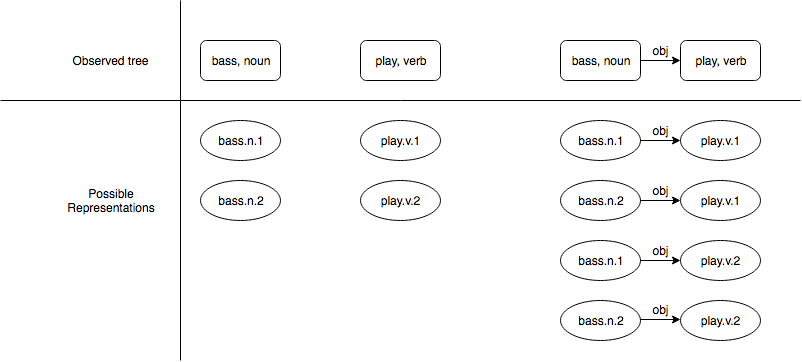
\includegraphics[width=\linewidth]{figure/poss_subtrees.png}
\caption{Illustration of the possible abstract representations for different subtrees of size one and two given the same dictionary of possible abstract representations..}
\label{fig:ast}
\end{figure}

\section{Splitting Calculations into Sub-Problems}
One way to reduce the computational complexity is to realize that in many cases the problem of estimating parameters often can be divided into several sub-problems, depending on the nature of the vocabulary sets, dictionary sets and the abstract set. In particular we consider sets $F$, and for each language $s$ $W_s$, $D_s$ that can be partitioned into subsets $F'$, $W'_s$, $D'_s$, $F''$, $W''_s$, $D''_s$, such that for any language, observation and abstract representation $s, x, y$
\begin{align*}
    (x,y)&\in D'_s, s\in S \implies x\in W'_s, y\in F'\\
    (x,y)&\in D''_s, s\in S \implies x\in W''_s, y\in F''.
\end{align*}
This means that if two words could possibly represent the same abstract function they must necceccarily be in the same partition and if two abstract functions can linearize to the same word they must neccessarily be in the same partition.

Assuming such a partition is possible we have that
\begin{equation*}
    x_{si}\in W'_s, y_j\in F'' \implies \phi^t_{sij}=P(X = x_{si}|Y = y_j)=0 \implies \hat c^t_{sij}=0,
\end{equation*}
for all $t$. Looking at equations \ref{eq:expected_counts} and \ref{eq:em_update} it is now easy to see that for any $s,i,j$ such that $x_i \in W'_s, y_j\in F'$ and any $k,l,m$ such that $x_l \in W''_k, y_m\in F''$, the updated parameters corresponding to observations and abstract representations in the first set of partitions $\pi^t_j, \phi^t_{sij}$ will not depend on parameters corresponding to the second set of partitions $\pi^{t-1}_m, \phi^{t-1}_{klm}$ and vice versa. This means that all calculations can be done separately for each of the two partitions. This kind of division into sub problems can of course be done recursively by applying the same procedure iteratively on the partitioned sets in order to ultimately divide the problem into a set of minimal sub problems.

In the setup used in the experiments we have used that the part of speech tag for each word in a dependency tree is known, meaning that given a bigram with a verb as the head and a noun as the dependent the abstract representation must necessarily have abstract functions of those two categories. In the setup where dependency labels are used and incorporated in the abstract representation these also further allow partitioning, as all observations of bigrams with a certain dependency label must necessarily be represented by an abstract representation containing the same dependency label.

Cursory experiments showed that for the wordnet dictionaries, attempts of further partitioning apart from the use of the obvious partitions mentioned above likely were to get very small gains as soon as several languages were used for estimation. This because almost all of the synsets within one word class would be in one large partition. Due to this, no investigation was done to do further partitioning.

\section{Merged Wordnet}
\label{section:cluster}
To reduce the size of the abstract function set a custom dictionary of possible abstract representations based on wordnet was compiled where abstract representations of each word was composed of merged clusters of wordnet synsets. These clusters were made by using the hypernym relations defined for nouns and verbs in wordnet such that rarely seen synsets were merged together with other rare synsets that share the same hypernym. For example a possible such merge would be to take the two rarely seen synsets corresponding to the fishes bass and trout, bass.n.1 and trout.n.1, and merge them into their common hypernym synset fish.n.1. As can be seen in figure \ref{fig:clust_poss_tree}, representing the two fishes with a common synset will as a result also make the two subtrees (bass, obj, eat) and (trout, obj, eat) share a common abstract representation. 

The procedure for merging synsets is based on probabilities estimated using a unigram model based on the wordnet dictionary as described in the previous section, that is a model only looking at sub-trees of size one. These probabilities can be interpreted as estimations of the frequency with which each synset appears in text. Using these probabilities, the \emph{information content} of each synset is defined as
\begin{equation}
    I(y)=-\log\sum_{y'\in h(y)} P(y'),
\end{equation}
where $h(y_i)$ is the set of all subsumers in the hypernym hierarchy of $y_i$. This definition of synset information content is the same as the one used in \citep{resnik1995similarity}. An information cutoff $C$ is made and one cluster is created for each synset with an information content lower than $C$. All synsets with an information content higher than C are then assigned to the cluster represented by its subsumer subset with the highest information content lower that $C$. That is each synset $y$ is assigned to the cluster represented by $f(y)$ where
\begin{equation}
    f(y)=\argmax_{y'\in h(y), I(y')<C} I(y').
\end{equation}
A new abstract function set and new dictionary sets can now be constructed by replacing each abstract function in the wordnet dictionary with the clustered representation of that synset.
\begin{figure}[!htbp]
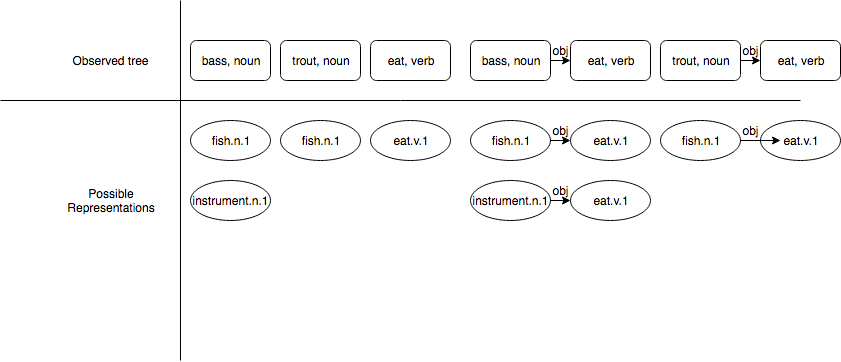
\includegraphics[width=\linewidth]{figure/clust_poss_subtrees.png}
\caption{Illustration of the possible abstract representations for different subtrees using the clustered dictionary. Note that both the words trout and bass point to the cluster fish.n.1 allowing us to capture the information that fish are something that often are the object of eat from a a wider range of observations.}
\label{fig:ast}
\end{figure}
\section{Data Sources and Parsing}
The data used to estimate the parameters for the probabilistic model is the automatically parsed training data used for CoNLL 2017 shared task \citep{ginter2017conll}. This data has been dependency parsed with the tool UDPipe and come in CoNNL-U format. From the parsed trees all subtrees of size two was counted using the lemma, part of speech tag and the dependency relation between the two nodes for each language separately. For each of the dictionaries used all subtrees containing unknown words was discarded, since many trees contained nonsense words likely originating from faulty parsing by the Common Crawl, which is one of the data sources used for the CoNLL 2017 data.

\section{Evaluation Models}
\label{sec:models}

For evaluation purposes, five variations of the basic model was defined. First, in order to assign probabilities for bigrams not observed in the training data, two different backoff strategies was chosen. In the first model, we utilized \textbf{stupid backoff}, introduced by \citet{brants2007large}. Stupid backoff doesn't define a normalized probability, but the ``score'' for one bigram is defined as following:

\begin{equation*}
S(\text{word} | \text{head}) = \begin{cases}
\frac{\text{count(word, head})}{\text{count}(\text{head})} & \text{if count(word, head)} > 0\\[.5em]
\lambda \cdot \frac{\text{count(word)}}{N} & \text{otherwise},
\end{cases}
\end{equation*}
where $N$ is the total number of counts and $\lambda=0.4$ a standard backoff constant. This is a very simple and memory-effective smoothing method, and it has been show to approach state-of-the-art methods such as Kneser-Nay smoothing in large-scale models \citep{brants2007large}.

The second model is an interpolation model which also has been shown to yield good results \citep{chen1996empirical}. It is a linear combination between the unigram and bigram together with the part-of-speech bigram and unigram. The score for a example bigram in this model is defined as follows:

\begin{align*}
    S(\text{football}|\text{play}) &= \lambda_0 P(\text{football}|\text{play}) + \lambda_1
    P(\text{football}) \\ &+ \lambda_2
    P(\text{noun}|\text{verb}) + \lambda_3
    P(\text{noun}),
\end{align*}
with the interpolation constants set to $\lambda_0 = 0.4$ and $\lambda_1=\lambda_2=\lambda_3=0.2$.

Except for these two models, we also created a variant where the bigram models is not only conditioned on the abstract function of the head, but also the dependency relation label between the dependent and the head node in the tree. This means that the stupid backoff model is updated as follows:

\begin{equation*}
S(\text{word} | \text{head}, \text{deprel}) = \begin{cases}
\frac{\text{count(word, head, deprel})}{\text{count}(\text{head, deprel})} & \text{if count(word, head, deprel)} > 0\\[.5em]
\lambda \cdot \frac{\text{count(word)}}{N} & \text{otherwise},
\end{cases},
\end{equation*}
with $N$ and $\lambda=0.4$ as before. The interpolation model was extended in a similar way, which means that we in total have five variations on our model:
\begin{enumerate}
    \item Unigram.
    \item Bigram with stupid backoff.
    \item Bigram with stupid backoff and dependency relation label.
    \item Interpolation.
    \item Interpolation with dependency relation label.
\end{enumerate}
